\chapter {Execução dos Testes e Análise dos Resultados}

Nesse capítulo vamos descrever o ambiente onde os testes foram realizados, as métricas que foram escolhidas para medir a performance e os resultados obtidos.

\section{Ambiente de testes}

Os testes foram realizados em uma máquina virtualizada, via VirtualBox, com as seguintes configurações:

\begin{itemize}
\item Sistema Operacional: Debian GNU/Linux 6.0
\item Processador: 1 
\item Quantidade de Memória RAM: 4 GB
\item MongoDB: Versão 2.4.0 padrão
\item PostgreSQL: Versão 8.4.16 padrão
\item Driver Python MongoDB: pymongo
\item Driver Python PostgreSQL: psycopg
\end{itemize}

\section{Massa de Dados}

Conforme Molyneaux diz ~\cite{theartoftestperf}, a importância de prover a quantidade de dados de qualidade para um teste não pode ser exagerada. Segundo ele a quantidade e a qualidade dos dados podem definir o sucesso ou insucesso dos testes. Para o nosso projeto foi desenvolvido um script em python para a geração da massa de dados. Os dados podem tanto ser inseridos diretamente na base de dados quanto em arquivos CSV que serão utilizados durante os testes. Os arquivos utilizados nos testes possuem tamanho médio de 400 KB. A quantidade de dados gerados também pode ser configurada pelo seguinte:

\begin{enumerate}
	\item Quantidade de Unidades Pagadoras (Orgãos);
	\item Quantidade de empregados por orgão;
	\item Quantidade de dependentes por empregado;
	\item Quantidade de documentos por empregado;
	\item Quantidade de documentos por dependente;
\end{enumerate}

A quantidade de dados utilizados pode ser vista na tabela \ref{tab:massadadosutil}

\begin{table}
	\caption{Massa de Dados Utilizada}
	\begin{center}
	\begin{tabularx}{\textwidth}{ | c | X | }
	\hline
		\textbf{Quantidade de Unidades Pagadoras} & \multicolumn{1}{c|}{\textbf{Descrição}} \\
	\hline
		Quantidade de empregados por orgão & 10\\
	\hline 
		Quantidade de dependentes por empregado & 100 \\
	\hline
		Quantidade de documentos por empregado & 5\\
	\hline
		Quantidade de documentos por dependente & 2\\
	\hline
	\hline
		Quantidade de dependentes excluídos & 500\\
	\hline
	\hline
		Quantidade de empregados desligados & 250\\
	\hline
	\end {tabularx}
	\end{center}
	\label{tab:massadadosutil}
\end{table}

\section{Métricas}

Quando se quer balancear o custo e a performance, todos os envolvidos na produção do software se preocupam com a execução de testes de performance. A avaliação de performance é necessária em todas as etapas do ciclo de vida de software e é requerida sempre que o arquiteto precisa comparar alternativasv~\cite{rajjain}. Em um teste de performance a escolha das métricas é de grande importância. Segundo Raj Jain ~\cite{rajjain}, escolher as métricas erradas é um dos erros mais comuns. Para o nosso trabalho as métricas escolhidas foram a vazão e o tempo de resposta.

\section{Resultados}

\subsection{Insere Órgãos}

\begin{figure}[!htbp]
	\begin{center}
		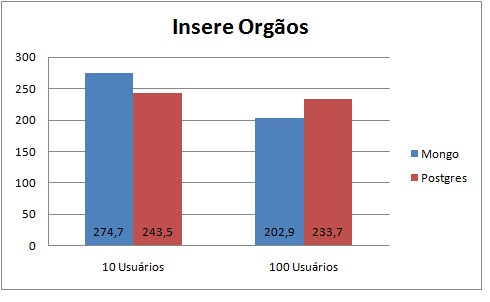
\includegraphics[width=0.8\textwidth]{resultados/insere_orgaos}
	\end{center}
	\caption{Resultados - Insere Órgãos}
	\label{fig:resultinsereorgaos}
\end{figure}

\subsection{Insere Empregados}

\begin{figure}[!htbp]
	\begin{center}
		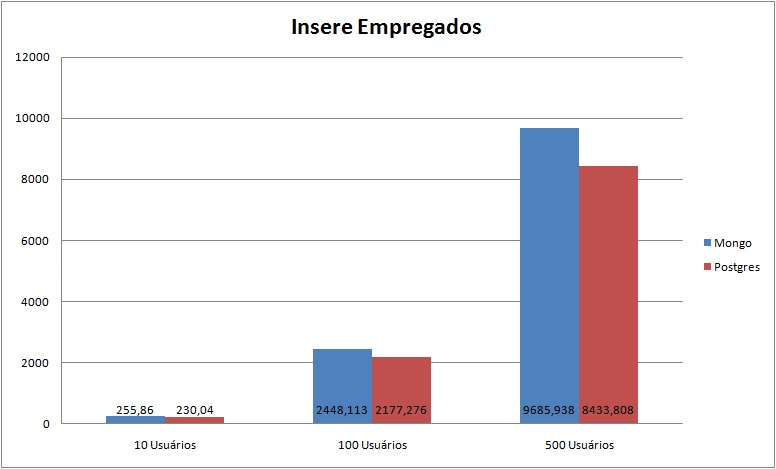
\includegraphics[width=0.8\textwidth]{resultados/insere_empregados}
	\end{center}
	\caption{Resultados - Insere Empregados}
	\label{fig:resultinsereempregados}
\end{figure}

\subsection{Insere Dependentes}

\begin{figure}[!htbp]
	\begin{center}
		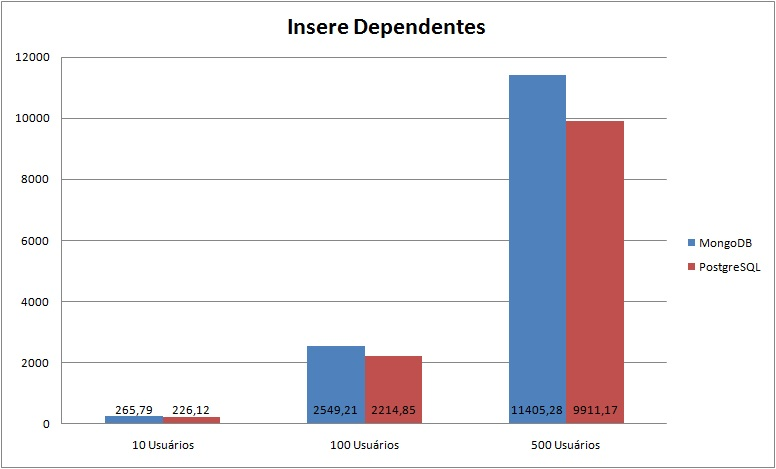
\includegraphics[width=0.8\textwidth]{resultados/insere_dependentes}
	\end{center}
	\caption{Resultados - Insere Dependentes}
	\label{fig:resultinseredependentes}
\end{figure}

\subsection{Insere Documento do Empregado}

\begin{figure}[!htbp]
	\begin{center}
		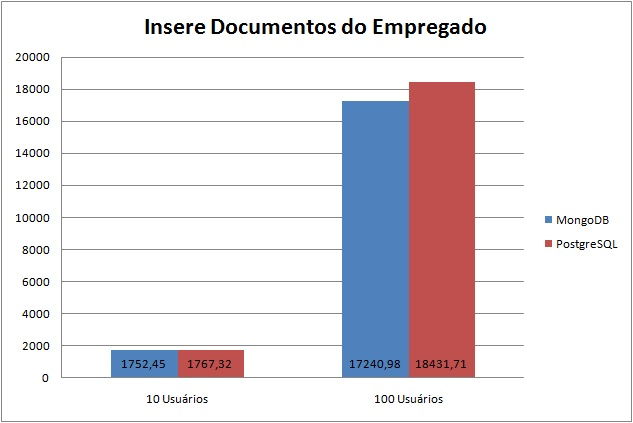
\includegraphics[width=0.8\textwidth]{resultados/insere_doc_empregado}
	\end{center}
	\caption{Resultados - Insere Documento do Empregado}
	\label{fig:resultinseredocempregado}
\end{figure}

\subsection{Insere Documento do Dependente}

\begin{figure}[!htbp]
	\begin{center}
		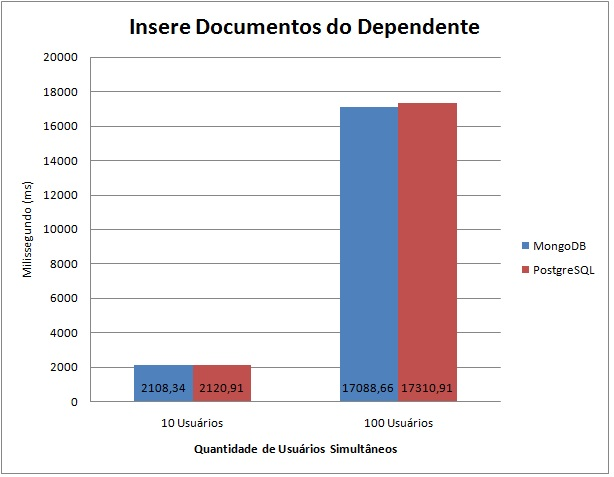
\includegraphics[width=0.8\textwidth]{resultados/insere_doc_dependentes}
	\end{center}
	\caption{Resultados - Insere Documento do Dependente}
	\label{fig:resultinseredocdependente}
\end{figure}

\subsection{Lista Órgãos}

\begin{figure}[!htbp]
	\begin{center}
		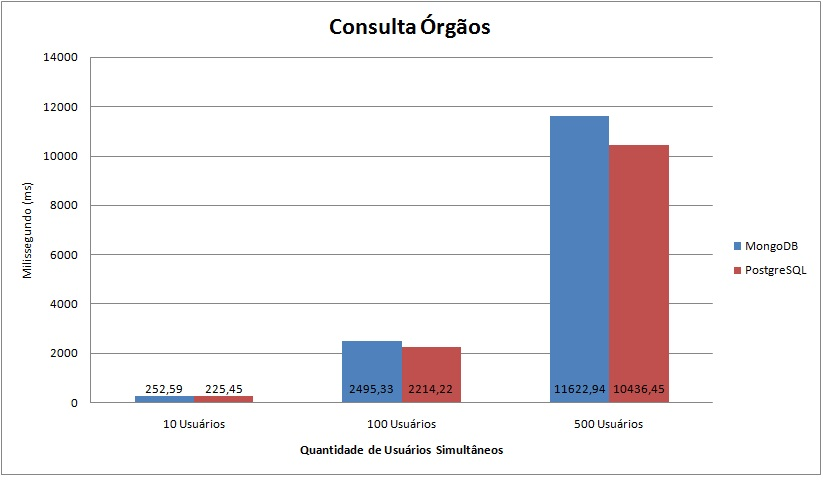
\includegraphics[width=0.8\textwidth]{resultados/consulta_orgaos}
	\end{center}
	\caption{Resultados - Lista Órgãos}
	\label{fig:resultlistaorgaos}
\end{figure}

\subsection{Lista Empregados}

\begin{figure}[!htbp]
	\begin{center}
		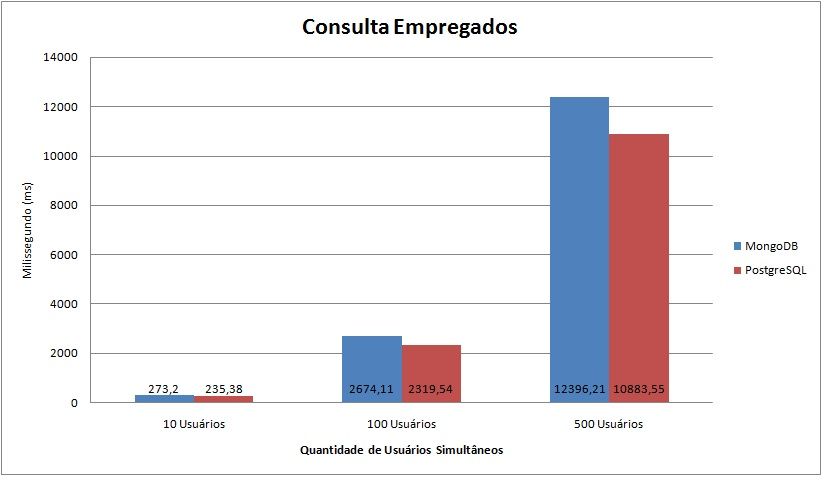
\includegraphics[width=0.8\textwidth]{resultados/consulta_empregados}
	\end{center}
	\caption{Resultados - Lista Empregados}
	\label{fig:resultlistaempregados}
\end{figure}

\subsection{Lista Documentos do Empregado}

\begin{figure}[!htbp]
	\begin{center}
		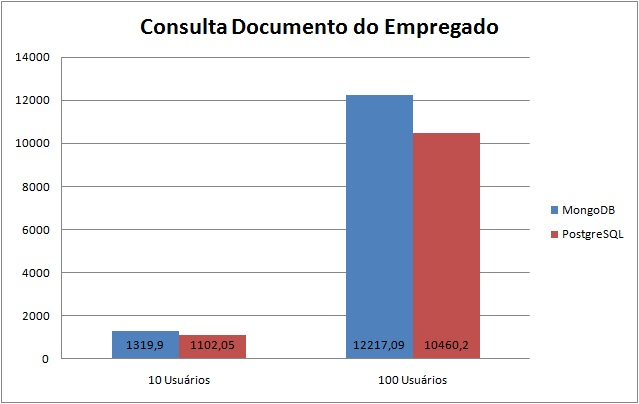
\includegraphics[width=0.8\textwidth]{resultados/consulta_doc_empregado}
	\end{center}
	\caption{Resultados - Lista Documentos do Empregado}
	\label{fig:resultlistadocempregado}
\end{figure}

\subsection{Lista Documentos do Dependente}

\begin{figure}[!htbp]
	\begin{center}
		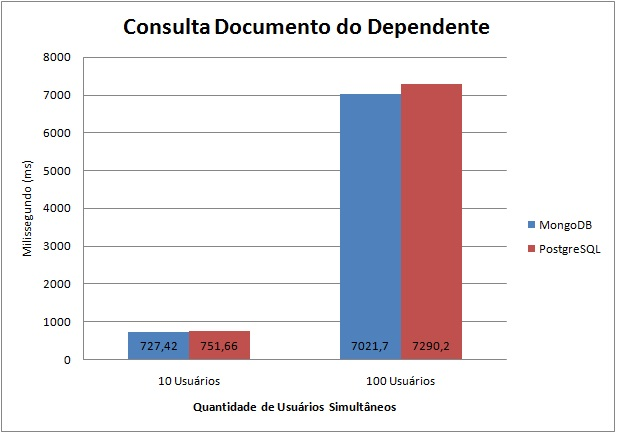
\includegraphics[width=0.8\textwidth]{resultados/consulta_doc_dependente}
	\end{center}
	\caption{Resultados - Lista Documentos do Dependente}
	\label{fig:resultlistadocdependente}
\end{figure}

\subsection{Consulta Empregados Ativos}

\begin{figure}[!htbp]
	\begin{center}
		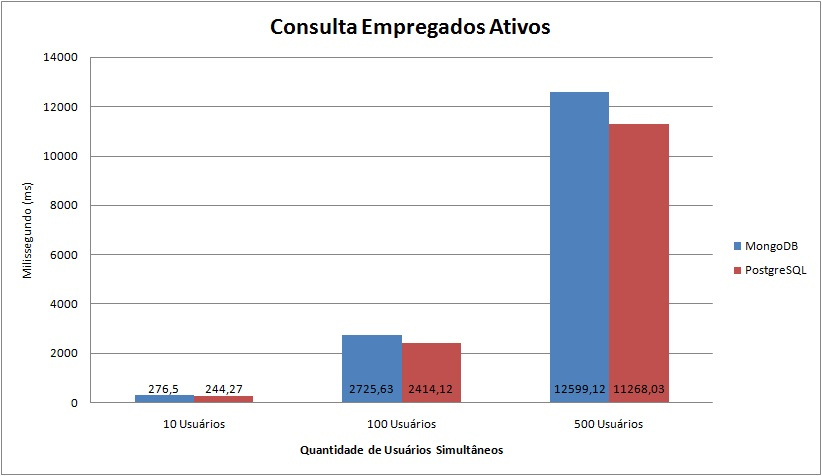
\includegraphics[width=0.8\textwidth]{resultados/consulta_estatistica}
	\end{center}
	\caption{Resultados - Consulta Empregados Ativos}
	\label{fig:resultlistaempregadosativos}
\end{figure}

\subsection{Remove Dependentes}


\subsection{Desliga Empregado}


